\documentclass{article}
\input{tex/00_preambule.tex}

\author{Artur Radwański}
\title{Zagadnienie Lagrange'a}
\setDepartment{Wydział Informatyki}
\setFaculty{Elektronika i Telekomunikacja}
\setSupervisor{Grupa 4}

\begin{document}

\maketitle
% \input{tex/02_student_declaration}
% \input{tex/03_engineering_thesis_outline}

% \null
% \newpage
% \null
% \newpage

\linespread{1.3}
\selectfont

\section{System}
\begin{itemize}
    \item Procesor: AMD Ryzen 7 9800x3d
    \item System operacyjny: 6.19.9-arch1-1 (Linux)
    \item Język programowania: c++23
    \item Kompilator: gcc version 15.2.1 20260209 (GCC) 
\end{itemize}

\section{Zadanie}
\subsection{Cel}
Celem zadania było zbadanie jak rozmieszczenie węzłów interpolacji wpływa na dokładność przybliżenia oraz porównanie podejścia Lagrange'a oraz metody ilorazów różnicowych.
\subsection{Realizacja}

W celu zbadania właściwości numerycznych wybranych metod interpolacji, zaimplementowano środowisko testowe w języku C++, pozwalające na automatyczne porównanie wyników dla zmiennej liczby węzłów $n \in [1, 30]$. Proces badawczy zrealizowano w następujących krokach:

\begin{enumerate}
    \item \textbf{Generowanie węzłów interpolacji:} Dla każdego stopnia wielomianu wyznaczono dwa zestawy punktów w przedziale $[a, b]$:
    \begin{itemize}
        \item \textbf{Węzły równoodległe:} wyznaczane przy stałym kroku $h = \frac{b-a}{n}$,
        \item \textbf{Węzły Czebyszewa:} będące zerami wielomianów Czebyszewa, przeskalowane z przedziału $[-1, 1]$ do $[a, b]$
    \end{itemize}
    
    \item \textbf{Implementacja algorytmów:}
    \begin{itemize}
        \item \textbf{Metoda Lagrange'a:} Wykorzystano klasyczną postać bazową wielomianu. Wartość w każdym punkcie pomiarowym obliczana była bezpośrednio ze wzoru sumacyjnego.
        \item \textbf{Metoda Newtona:} Zastosowano podejście oparte na ilorazach różnicowych. Współczynniki wielomianu obliczane były jednorazowo dla danego zestawu węzłów, a następnie wykorzystywane do efektywnego wyznaczania wartości wielomianu przy użyciu schematu Hornera.
    \end{itemize}

    \item \textbf{Analiza błędów:} Dla każdego zestawu danych przeprowadzono próbkowanie w 1000 punktach kontrolnych rozmieszczonych równomiernie. Jako miary dokładności przyjęto:
    \begin{itemize}
        \item \textbf{Błąd kwadratowy ($E_{sqr}$):} dający obraz ogólnego dopasowania funkcji na całym przedziale.
        \item \textbf{Błąd maksymalny ($E_{max}$):} kluczowy dla zaobserwowania oscylacji brzegowych (efektu Rungego).
    \end{itemize}
\end{enumerate}
\newpage
\section{Wyniki}
\begin{table}[htbp]
\centering
\caption{Porównanie błędów maksymalnych ($E_{max}$) dla różnych metod i rozmieszczenia węzłów.}
\label{tab:max_error}
\begin{tabular}{@{}ccccc@{}}
\toprule
\textbf{n} & \textbf{Newton (Równ.)} & \textbf{Newton (Czeb.)} & \textbf{Lagrange (Równ.)} & \textbf{Lagrange (Czeb.)} \\ \midrule
3          & 19,3037                 & 27,5937                 & 19,3037                   & 27,5937                   \\
4          & 22,8386                 & 23,6327                 & 22,8386                   & 23,6327                   \\
5          & 31,5114                 & 21,1816                 & 31,5114                   & 21,1816                   \\
6          & 19,3037                 & 29,2052                 & 19,3037                   & 29,2052                   \\
7          & 26,2011                 & 21,9105                 & 26,2011                   & 21,9105                   \\
8          & 35,9706                 & 26,3311                 & 35,9706                   & 26,3311                   \\
9          & 81,0228                 & 26,0274                 & 81,0228                   & 26,0274                   \\
10         & 119,054                 & 24,2327                 & 119,054                   & 24,2327                   \\ \midrule
15         & 576,223                 & 7,95133                 & 576,223                   & 7,95133                   \\
20         & 165,596                 & 0,56267                 & 165,596                   & 0,56267                   \\
25         & 8,81373                 & 0,00427                 & 8,81373                   & 0,00427                   \\
29         & 0,33825                 & 4,35e-05                & 0,33825                   & 4,35e-05                  \\ \bottomrule
\end{tabular}
\end{table}

\begin{table}[htbp]
\centering
\caption{Porównanie średniego błędu kwadratowego ($E_{sqr}$) dla różnych metod interpolacji.}
\label{tab:mse_error}
\begin{tabular}{@{}ccccc@{}}
\toprule
\textbf{n} & \textbf{Newton (Równ.)} & \textbf{Newton (Czeb.)} & \textbf{Lagrange (Równ.)} & \textbf{Lagrange (Czeb.)} \\ \midrule
3          & 0,23246                 & 0,27919                 & 0,23246                   & 0,27919                   \\
4          & 0,29254                 & 0,26257                 & 0,29254                   & 0,26257                   \\
5          & 0,32873                 & 0,22232                 & 0,32873                   & 0,22232                   \\
6          & 0,23246                 & 0,32609                 & 0,23246                   & 0,32609                   \\
7          & 0,32041                 & 0,24313                 & 0,32041                   & 0,24313                   \\
8          & 0,38760                 & 0,26476                 & 0,38760                   & 0,26476                   \\
9          & 0,72687                 & 0,25528                 & 0,72687                   & 0,25528                   \\
10         & 0,96395                 & 0,23868                 & 0,96395                   & 0,23868                   \\ \midrule
15         & 3,52828                 & 0,10615                 & 3,52828                   & 0,10615                   \\
20         & 0,85074                 & 0,00959                 & 0,85074                   & 0,00959                   \\
25         & 0,03916                 & 5,87e-05                & 0,03916                   & 5,87e-05                  \\
29         & 0,00137                 & 5,64e-07                & 0,00137                   & 5,64e-07                  \\ \bottomrule
\end{tabular}
\end{table}

\subsection{Analiza występowania i niwelowania efektu Rungego}

Na podstawie danych z (Tab. \ref{tab:max_error} i \ref{tab:mse_error}) zaobserwowano efekt Rungego dla
węzłów równoodległych. Zjawisko to, polegające na nieliniowym wzroście oscylacji wielomianu przy krańcach przedziału, osiągnęło swoje apogeum dla $n=15$,
gdzie błąd maksymalny wyniósł aż $E_{max} \approx 576,22$. 

Tak wysoka wartość błędu świadczy o gwałtownych oscylacjach przybliżenia funkcji w obszarach brzegowych przy zastosowaniu równomiernego
rozkładu punktów. Warto zauważyć, że dla niskich rzędów ($n < 8$) błędy obu metod były zbliżone, jednak powyżej tej granicy błąd dla węzłów równoodległych zaczął
gwałtownie rosnąć.

Zastosowanie węzłów Czebyszewa w tym samym punkcie pomiarowym ($n=15$) pozwoliło na redukcję błędu maksymalnego do poziomu $7,95$ (ponad 70-krotna poprawa).
Choć dla tej konkretnej funkcji błąd Czebyszewa dla niskich $n$ jest początkowo wyższy niż w przypadku węzłów równoodległych, to jako jedyny gwarantuje on
stabilną zbieżność wraz ze wzrostem stopnia wielomianu. Już przy $n=29$ węzły Czebyszewa osiągają precyzję rzędu $10^{-5}$, podczas gdy węzły równoodległe nadal
generują błąd na poziomie $0,33$.

\begin{figure}[H]
    \centering
        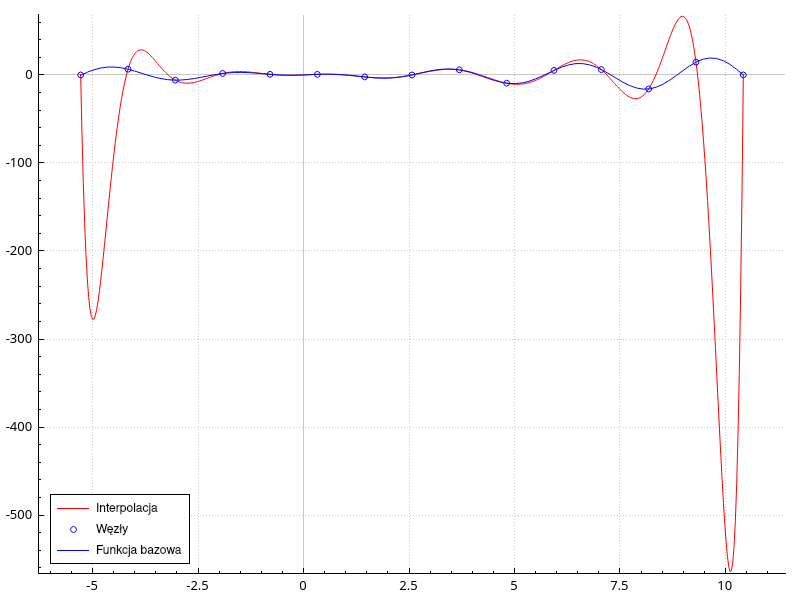
\includegraphics[width=0.8\textwidth]{img/rownomierne.png}
        \caption{Interpolacja z równoodległymi węzłami (n=15)}
        \label{fig:even}
\end{figure}

\begin{figure}[H]
    \centering
        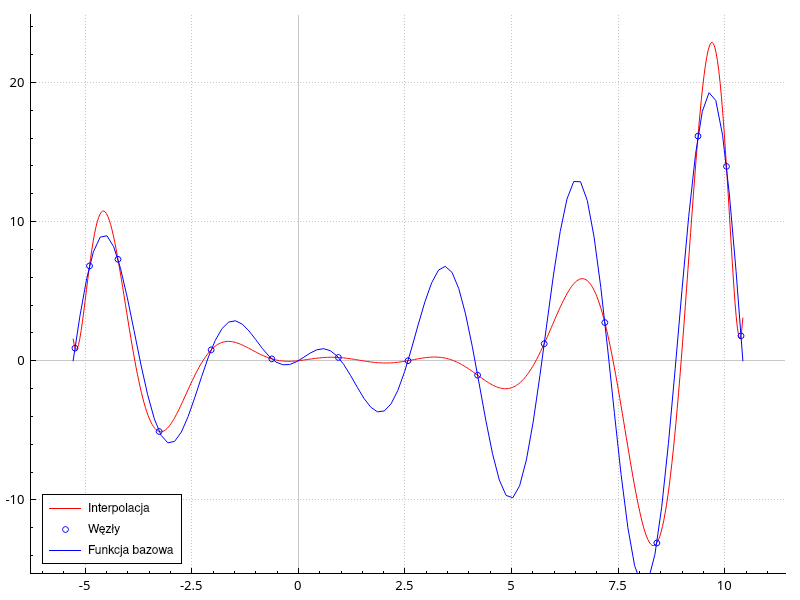
\includegraphics[width=0.8\textwidth]{img/czebyszew.png}
        \caption{Interpolacja z węzłami czebyszewa (n=15)}
        \label{fig:chebyshev}
\end{figure}

\subsection{Analiza przybliżeń dla $n=15$}

Porównanie przebiegów funkcji interpolujących z funkcją oryginalną $f(x)$ dla 15 węzłów (Rys. \ref{fig:even} i \ref{fig:chebyshev}) pozwala na bezpośrednią ocenę
jakości dopasowania modelu w różnych obszarach przedziału:

\begin{itemize}
    \item \textbf{Interpolacja na węzłach równoodległych:}
    Wykres wyraźnie ukazuje niepożądane zachowanie wielomianu w pobliżu krańców przedziału. Mimo że w centralnej części przedziału funkcja
    interpolująca niemal pokrywa się z oryginałem, to przy brzegach obserwujemy gwałtowne oscylacje, których amplituda przekracza 500 jednostek. Wielomian "ucieka"
    od funkcji bazowej, próbując wymusić przejście przez skrajne punkty, co w efekcie generuje
    ogromne rozbieżności.

    \item \textbf{Interpolacja na węzłach Czebyszewa:}
    W przeciwieństwie do poprzedniego przypadku, wykres dla węzłów Czebyszewa wykazuje stabilne dopasowanie na całym badanym zakresie. Dzięki zagęszczeniu węzłów
    przy krańcach przedziału, oscylacje brzegowe zostały stłumione, kosztem gorszego dopasowania w okolicach środka przedziału. Ze względu na bardziej równomierne
    rozłożenie błędu interpolacji, ten wielomian stanowi znacznie lepsze przybliżenie funkcji bazowej w praktyce.

\end{itemize}

\subsection{Stabilność numeryczna}
\begin{table}[htbp]
\centering
\caption{Porównanie maksymalnego błędu ($E_{max}$) dla wyższych stopni wielomianu.}
\label{tab:max_error_high}
\begin{tabular}{@{}ccccc@{}}
\toprule
\textbf{n} & \textbf{Newton (Równ.)} & \textbf{Newton (Czeb.)} & \textbf{Lagrange (Równ.)} & \textbf{Lagrange (Czeb.)} \\ \midrule
30          & 0.19454                 & 2.07627e-05             & 0.19454                   & 2.07629e-05              \\
40          & 5.61227e-06             & 8.5262e-06              & 5.75229e-06               & 1.35247e-11              \\
50          & 3.3836e-05              & 8.65939e-05             & 0.00163198                & 2.84217e-14              \\
60          & 0.14655                 & 0.00112684              & 1.96578                   & 3.19744e-14              \\
70          & 58.641                  & 4.20032                 & 1364.23                   & 2.57572e-14              \\
80          & 23280.2                 & 3.87708e+06              & 769083                   & 4.61853e-14              \\ \bottomrule
\end{tabular}
\end{table}

Analiza danych przedstawionych w Tabeli \ref{tab:max_error_high} pozwala na wyciągnięcie kluczowych wniosków dotyczących odporności badanych algorytmów na błędy zaokrągleń przy bardzo wysokich stopniach wielomianu ($n \in [30, 80]$):

\begin{enumerate}
    \item \textbf{Załamanie stabilności metody Newtona:} 
    Do wartości $n=40$ metoda Newtona (oparta na ilorazach różnicowych) zachowuje relatywną stabilność. Interpolowanie tą metodą dla większej ilości węzłów
    przestaje mieć sens, ponieważ błąd zaczyna rosnąć wraz ze stopniem wielomianu.

    \item \textbf{Dobra stabilność postaci Lagrange'a:}
    Najbardziej zaskakującym wynikiem jest zachowanie algorytmu Lagrange'a w połączeniu z węzłami Czebyszewa. Podczas gdy wszystkie inne kombinacje metod i
    węzłów zawodzą powyżej $n=70$, ta konkretna para utrzymuje błąd kwadratowy na stałym, minimalnym poziomie rzędu $10^{-14}$.

    \item \textbf{Wpływ rozmieszczenia węzłów na błędy maszynowe:}
    Dane pokazują, że węzły Czebyszewa nie tylko niwelują efekt Rungego, ale również znacząco przesuwają granicę stabilności numerycznej. Dla $n=80$ błąd
    metody Lagrange'a na węzłach równoodległych ($7,6 \cdot 10^5$) w porównaniu do węzłów Czebyszewa
    ($4,6 \cdot 10^{-14}$) wykazuje różnicę aż 19 rzędów wielkości, natomiast metoda Newtona dawała mniejszy błąd maksymalny nawet dla n=70.

    \item \textbf{Praktyczna granica interpolacji wielomianowej:}
    Wyniki dla $n=80$ (błędy rzędu $10^4 - 10^5$) jednoznacznie wskazują, że bez specjalnej implementacji sprzętowej (lub symulacji
    w oprogramowaniu) zwiększonej preycyzji liczb, taka interpolacja jest niepraktyczna.
\end{enumerate}

\section{Wnioski}

Przeprowadzone badania nad interpolacją wielomianową funkcji $f(x)$ pozwoliły na sformułowanie następujących konkluzji:

\begin{enumerate}
\item \textbf{Kluczowa rola rozmieszczenia węzłów:} Wybór punktów interpolacji okazał się czynnikiem ważniejszym niż sam wybór algorytmu (Newton vs Lagrange).
Węzły równoodległe, prowadzą do wystąpienia silnego \textbf{efektu Rungego}, który przy n=15 generuje błędy przekraczające
20-krotność amplitudy funkcji. Zastosowanie \textbf{węzłów Czebyszewa} skutecznie eliminuje te oscylacje, zapewniając stabilną zbieżność przybliżenia wraz ze
wzrostem stopnia wielomianu.

\item \textbf{Stabilność numeryczna metod:} Do stopnia $n \approx 30$ obie badane metody (Newtona i Lagrange'a) są równoważne. Jednakże przy
ekstremalnie wysokich rzędach ($n > 60$), postać Newtona oparta na ilorazach różnicowych ulega załamaniu ze względu na kumulację błędów zaokrągleń maszynowych
(osiągając błąd rzędu $10^6$ dla $n=80$). W tych samych warunkach \textbf{metoda Lagrange'a na węzłach Czebyszewa} zachowuje precyzję, co czyni ją najbardziej stabilnym rozwiązaniem dla wielomianów wysokiego stopnia.

\item \textbf{Charakterystyka błędów:} Porównanie metryk $E_{max}$ oraz $E_{sqr}$ wykazało, że błąd średniokwadratowy może być mylący w ocenie jakości interpolacji,
gdyż "maskuje" gigantyczne rozbieżności występujące na brzegach przedziału.

\item \textbf{Zalecenia implementacyjne:} Na podstawie uzyskanych wyników, do systemów wymagających wysokiej precyzji przy dużym $n$ najlepiej stosować
wielomian Lagrange'a w połączeniu z węzłami Czebyszewa. Metoda Newtona pozostaje jednak bardziej efektywna w scenariuszach dynamicznych
(gdzie liczba węzłów ulega zmianie w trakcie obliczeń), pod warunkiem zachowania umiarkowanego stopnia wielomianu ($n < 30$).

\end{enumerate}
\end{document}